

%----------------------------------------------------------------------------------------
%	PACKAGES AND OTHER DOCUMENT CONFIGURATIONS
%----------------------------------------------------------------------------------------

\documentclass[xcolor=x11names,compress]{beamer}
\usepackage{graphicx}
\usepackage[margin=5pt]{subfig}
\usepackage{tikz}
\usetikzlibrary{decorations.fractals}

\useoutertheme[subsection=false,shadow]{miniframes}
%\useoutertheme{default} % to remove top navigation bar
\useinnertheme{default}
\usefonttheme{serif}
\usepackage{palatino}

\setbeamerfont{title like}{shape=\scshape}
\setbeamerfont{frametitle}{shape=\scshape}
%\setbeamertemplate{caption}[]
\setbeamertemplate{navigation symbols}{}%remove navigation symbols
\setbeamercovered{transparent}

\setbeamercolor*{lower separation line head}{bg=DeepSkyBlue4}
\setbeamercolor*{normal text}{fg=black,bg=white} 
\setbeamercolor*{alerted text}{fg=red} 
\setbeamercolor*{example text}{fg=black} 
\setbeamercolor*{structure}{fg=black} 
 
\setbeamercolor*{palette tertiary}{fg=black,bg=black!10} 
\setbeamercolor*{palette quaternary}{fg=black,bg=black!10} 

%\setbeamertemplate{navigation symbols}{}%remove navigation symbols

\addtobeamertemplate{navigation symbols}{}{%
    \usebeamerfont{footline}%
    \usebeamercolor[fg]{footline}%
    \hspace{1em}%
    \insertframenumber/\inserttotalframenumber
}

\renewcommand{\(}{\begin{columns}}
\renewcommand{\)}{\end{columns}}
\newcommand{\<}[1]{\begin{column}{#1}}
\renewcommand{\>}{\end{column}}




\begin{document}


%----------------------------------------------------------------------------------------
%	TITLE SECTION 
%----------------------------------------------------------------------------------------

\begin{frame}
\title{Integration of a PXE based image publisher on the UForge platform}
\author
{
	Presented by \textbf{SID-LAKHDAR Riyane}\\
	(M1 MoSIG: ENSIMAG / UJF)\\
	Supervised by \textbf{BREMOND Joris}\\
	(Software Development Engineer: UShareSoft)\\
	\vspace{1cm}
	
\includegraphics[height=1.5cm,width=5.5cm]{logo/logo_usharesoft.png}
}
\date
{
	\vspace{1cm}
	\today
}
\titlepage
\end{frame}


%----------------------------------------------------------------------------------------
%	Motivation: the PXE technology for an image publisher 
%----------------------------------------------------------------------------------------
\begin{frame}{Motivation: the PXE technology for an image publisher}
\tableofcontents
\end{frame}



%----------------------------------------------------------------------------------------
% What is the PXE specification
%----------------------------------------------------------------------------------------
\section{\scshape What is the PXE specification?}
\begin{frame}{The PXE specification}
	PXE: Preboot Execution Environment
	\begin{itemize}[<+->]
		\item Standardized client-server environment (part of the UEFI standard)
		\item Boots a software assembly retrieved from a network
		\item Most frequent choice for operating system booting, installation and deployment.
	\end{itemize}
\end{frame}


%----------------------------------------------------------------------------------------
\begin{frame}{Technical principles}
	\centering \textbf{The PXE boot process}
	\begin{figure}[t]
	\begin{center}
%		\subfloat[Architecture]{\includegraphics[width=0.45\linewidth]{chart/PXE_basis.png}}
%		\subfloat[Flow data-gram]{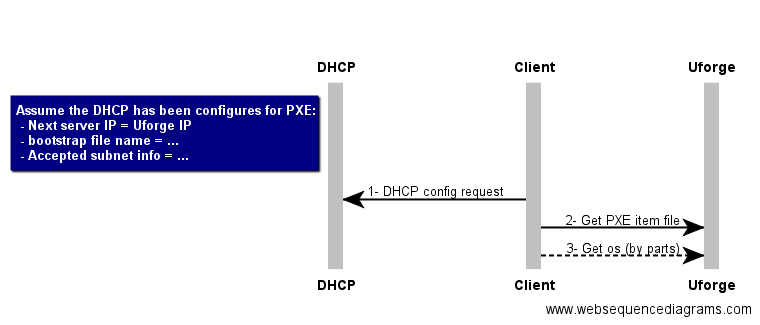
\includegraphics[width=0.45\linewidth]{chart/PXE_basis_datagram.png}}
		\subfloat{\includegraphics[width=0.9\linewidth]{chart/PXE_basis.png}}
	\end{center}
	\end{figure}


\end{frame}


%----------------------------------------------------------------------------------------
\begin{frame}{Technical principles}
	\centering \textbf{The PXE light client binary: iPXE}
	\begin{figure}[t]
	\begin{center}
		\subfloat{\includegraphics[width=0.9\linewidth]{chart/pxeBinary.png}}
	\end{center}
	\end{figure}


\end{frame}


%----------------------------------------------------------------------------------------
\begin{frame}{Limitations}
	The PXE boot process needs to fit
	\begin{itemize}
		\item \alert<+>
        {
			Network card ROM size
			\begin{figure}[t]
			\begin{center}
				\subfloat{\includegraphics[width=0.8\linewidth]{chart/limitation_NicRom.png}}
			\end{center}
			\end{figure}
		}
		\item Mandatory DHCP server configuration on the client network
		\item Client processor architecture
	\end{itemize}

\end{frame}


%----------------------------------------------------------------------------------------
\begin{frame}{Limitations}
	The PXE boot process needs to fit
	\begin{itemize}
		\item Network card ROM size
		\item \alert<+>
		{
			Mandatory DHCP server configuration on the client network
			\begin{figure}[t]
			\begin{center}
				\subfloat{\includegraphics[width=0.8\linewidth]{chart/limitation_dhcpConfiguration.png}}
			\end{center}
			\end{figure}
		}
		\item Client processor architecture
	\end{itemize}

\end{frame}


%----------------------------------------------------------------------------------------
\begin{frame}{Limitations}
	The PXE boot process needs to fit
	\begin{itemize}
		\item Network card ROM size
		\item Mandatory DHCP server configuration on the client network
		\item \alert<+>
		{
			Client processor architecture
			\begin{figure}[t]
			\begin{center}
				\subfloat{\includegraphics[width=0.8\linewidth]{chart/limitation_processorArchitecture.png}}
			\end{center}
			\end{figure}
		}
	\end{itemize}

\end{frame}


%Add the end of UForgePlatform scheme
%----------------------------------------------------------------------------------------
% Software architecture and features
%----------------------------------------------------------------------------------------
\section{\scshape UForge-integrated implementations  and architectures}
\frame{\tableofcontents[currentsection]}
\begin{frame}{First software architecture}
	\textbf{Straightforward client/UForge communication}
	\begin{figure}[t]
	\begin{center}
%		\subfloat[Architecture]{\includegraphics[width=0.45\linewidth]{chart/architecture_noIntermediary.png}}
%		\subfloat[Flow data-gram]{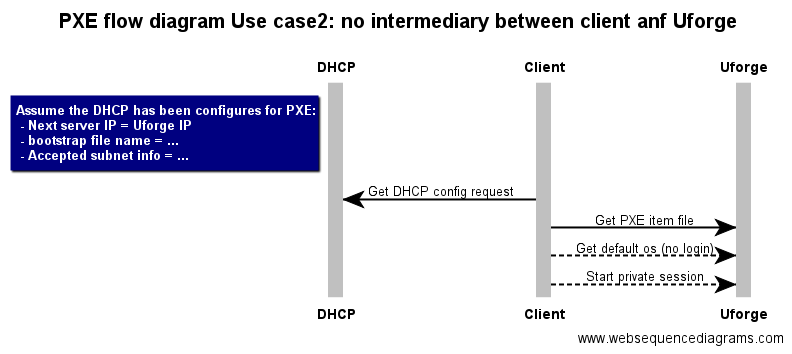
\includegraphics[width=0.45\linewidth]{chart/flowDiagram_noIntermediary.png}}
		\subfloat{\includegraphics[width=0.9\linewidth]{chart/architecture_noIntermediary.png}}
	\end{center}
	\end{figure}

\end{frame}


%----------------------------------------------------------------------------------------
\begin{frame}{Straightforward client/UForge communication}
	Advantages
	\begin{itemize}
		\item No \textbf{package} or tool to install on client network
		\item Any \textbf{upgrade} is offered without any intervention of the customer
		\item No need to any \textbf{connector} or specific tools for specific user processor or architecture
	\end{itemize}
\end{frame}


%----------------------------------------------------------------------------------------
\begin{frame}{Straightforward client/UForge communication}
	Drawbacks
	\begin{itemize}
		\item Limited set of features offered to the customer
        \item Creates useless contention on the UForge server and client network
        \item Don't take advantage of space and time locality
	\end{itemize}
\end{frame}


%----------------------------------------------------------------------------------------
\begin{frame}{Second software architecture}
	\textbf{Proxy on the client network}
	\begin{figure}[t]
	\begin{center}
%		\subfloat[Architecture]{\includegraphics[width=0.45\linewidth]{chart/architecture_proxy.png}}
%		\subfloat[Flow data-gram]{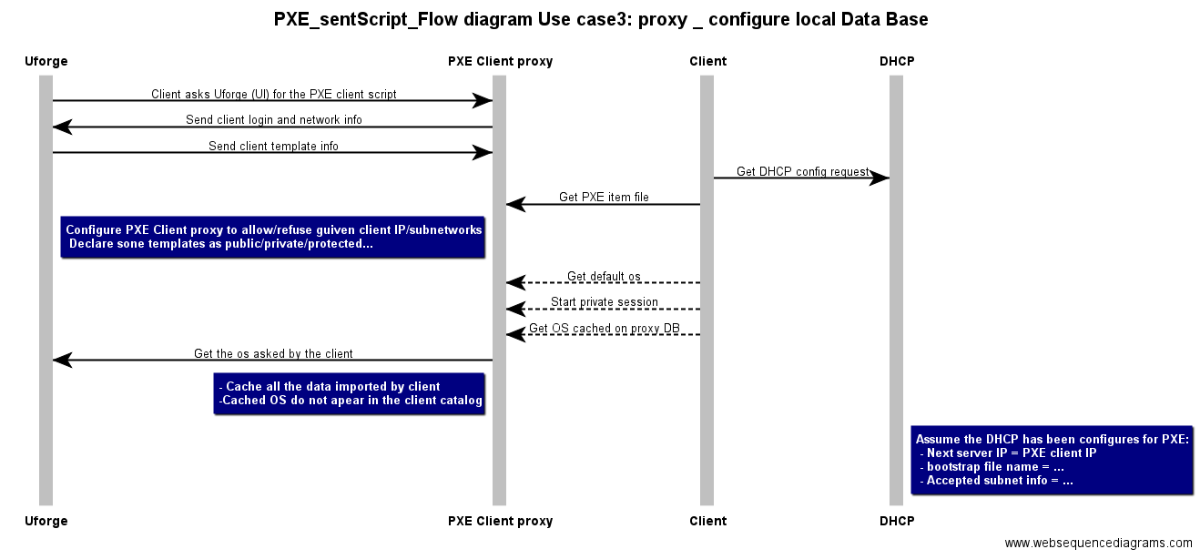
\includegraphics[width=0.45\linewidth]{chart/flowDiagram_proxy.png}}
		\subfloat{\includegraphics[width=0.9\linewidth]{chart/architecture_proxy.png}}
	\end{center}
	\end{figure}
\end{frame}


%----------------------------------------------------------------------------------------
%\begin{frame}{Proxy on the client network}
%	Drawbacks
%	\begin{itemize}
%		\item Requires a dedicated machine on the client network
%	\end{itemize}
%\end{frame}


%----------------------------------------------------------------------------------------
\begin{frame}{Demonstration}
	\begin{itemize}
		\item Straight forward UForge/Client communication
		\item 3 custom web services to answer all the PXE requests
		\item Set of tools to dynamically build the iPXE code for each request
		\item Custom PXE target format
	\end{itemize}
\end{frame}


%----------------------------------------------------------------------------------------
% Maintainability and evolution
%----------------------------------------------------------------------------------------
\section{\scshape Evolution and maintainability}
\frame{\tableofcontents[currentsection]}
\begin{frame}{Rethink the UForge design}

	\textbf{Modules based on services/aspects}
	\begin{figure}[t]
	\begin{center}
%		\subfloat[Architecture]{\includegraphics[width=0.45\linewidth]{chart/architecture_proxy.png}}
%		\subfloat[Flow data-gram]{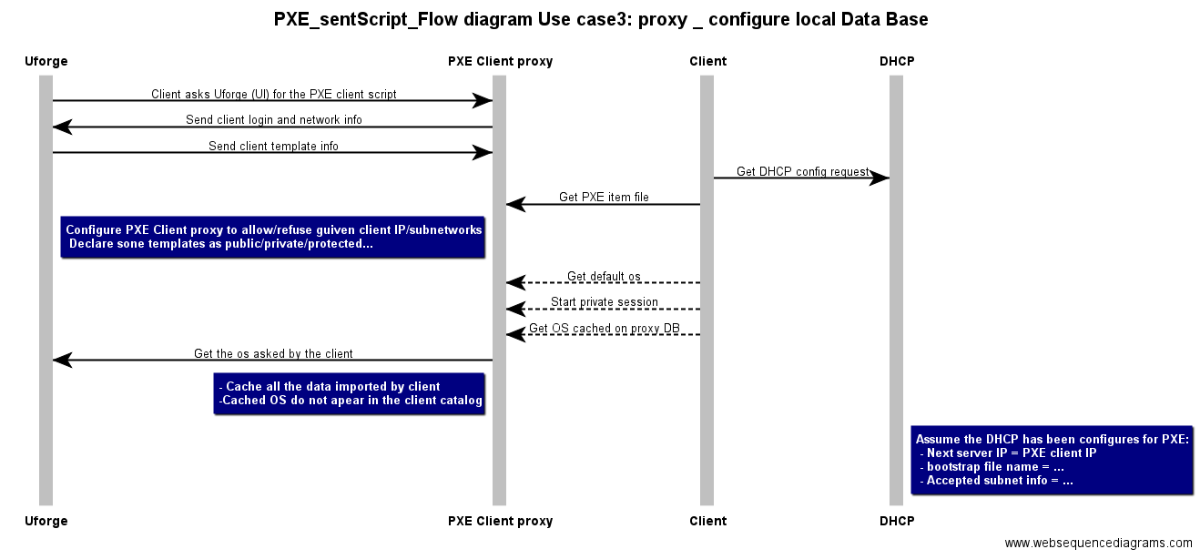
\includegraphics[width=0.45\linewidth]{chart/flowDiagram_proxy.png}}
		\subfloat{\includegraphics[width=0.9\linewidth]{chart/architecture_proxy.png}}
	\end{center}
	\end{figure}

\end{frame}


%----------------------------------------------------------------------------------------
\begin{frame}{Rethink the UForge design: module split}
	\begin{itemize}
		\item Split the UForge code in independent \textbf{modules}
		\item Delegate some services to modules deployed out of UForge
		\item Reduce contention on UForge: speed up image download
        	\begin{itemize}
				\item Network traffic
				\item Code concentration
			\end{itemize}
	\end{itemize}
\end{frame}


%----------------------------------------------------------------------------------------
\begin{frame}{Get ride of the connectors for each new cloud environment}
	\begin{itemize}
		\item Same publish process for all the light client environments and platforms
		\item Backup solution for buggy or nonexistent connectors
	\end{itemize}
\end{frame}


%----------------------------------------------------------------------------------------
\begin{frame}{Automatize machine installations}
	\begin{itemize}
		\item Open an image for a set of machines (sub networks)
		\item Get ride of UForge authentication for a set of machine deployment
	\end{itemize}
\end{frame}


%----------------------------------------------------------------------------------------
\begin{frame}{Other advantages}
	\begin{itemize}
		\item Get ride of the ISO format: Non user friendly boot process (external hard drive)
		\item Possible adaptations depending the client processors
		\item Upgrades and evolution require no customer intervention
	\end{itemize}
\end{frame}



%----------------------------------------------------------------------------------------
% Summary
%----------------------------------------------------------------------------------------
\begin{frame}{Summary}
	\begin{itemize}
		\item PXE: secure, user-friendly and efficient image publisher
		\item Get rides of the connector issue on heterogeneous host environment
		\item Get ride of customer intervention for any fix or upgrade
		\item Fits the current and future expectations of UShareSoft
	\end{itemize}
\end{frame}



%----------------------------------------------------------------------------------------
%	TITLE SECTION 
%----------------------------------------------------------------------------------------

\begin{frame}
\title{Integration of a PXE based image publisher on the UForge platform}
\author
{
	Thank you for your attention\\
	\vspace{2cm}
	
\includegraphics[height=1.5cm,width=5.5cm]{logo/logo_usharesoft.png}
}
\date
{
	\vspace{1cm}
	\today
}
\titlepage
\end{frame}

\end{document}